\documentclass{article}
%% Useful packages
\usepackage[utf8]{inputenc}
\usepackage[a4paper,left=2cm,right=2cm,top=2cm,bottom=2cm]{geometry}
\usepackage{crop,graphicx,amsmath,array,color,amssymb,fancyhdr,lineno}
\usepackage{flushend,stfloats,amsthm,chngpage,times,,lipsum,lastpage} 
\usepackage{calc,listings,color,wrapfig,tabularx,longtable,enumitem}
\usepackage[style=numeric-comp,backend=biber]{biblatex}
\addbibresource{Refs.bib}
\usepackage{lineno}
%%%%%%%%%%%%   Header and Footer  %%%%%%%%%%%%%
\pagestyle{fancy}
\fancypagestyle{plain}{%
  \renewcommand{\headrulewidth}{0pt}%
  \fancyhf{}%
}

\title{%
  First Assignment \\
  \large Equivalent representations of orientation matrices}
\author{Surname Name}

\begin{document}
\begin{titlepage}

\newcommand{\HRule}{\rule{\linewidth}{0.5mm}} % Defines a new command for the horizontal lines, change thickness here

%----------------------------------------------------------------------------------------
%	LOGO SECTION
%----------------------------------------------------------------------------------------
\center

\includegraphics[width=5cm]{Title/Unige-logo.jpeg}\\[1cm] % Include a department/university logo - this will require the graphicx package
 
%----------------------------------------------------------------------------------------

\center % Center everything on the page

%----------------------------------------------------------------------------------------
%	HEADING SECTIONS
%----------------------------------------------------------------------------------------

\textsc{\Huge Università degli studi di Genova}\\[1cm] % Name of your university/college
\textsc{\LARGE DIBRIS}\\[0.3cm]
\textsc{Department of Computer Science and Technology,}\\
\textsc{Bioengineering, Robotics and System Engineering}\\[1cm] % Minor heading such as course title
\textsc{\LARGE{Modeling and Control of Manipulators}}\\[1cm] % Major heading such as course name

%----------------------------------------------------------------------------------------
%	TITLE SECTION
%----------------------------------------------------------------------------------------
\makeatletter
\HRule \\[0.4cm]
{ \huge \bfseries First Assignment}\\[0.2cm] 
{\Large \bfseries Equivalent representations of orientation matrices}\\
% Title of your document
\HRule \\[1.5cm]
 
%----------------------------------------------------------------------------------------
%	AUTHOR SECTION
%----------------------------------------------------------------------------------------

\begin{minipage}{0.4\textwidth}
\begin{flushleft} \large
\emph{Author:}\\[0.2cm]
Balia Gian Marco\\
Polese Carolina\\
Salterini Filippo
\\[1.2em]
\emph{Student ID:}\\[0.2cm]
s4398275 \\
s4862903 \\
s4516129 \\[1.2em]
\end{flushleft}
\end{minipage}
~
\begin{minipage}{0.4\textwidth}
\begin{flushright} \large
\emph{Professors:} \\[0.2cm]
Giovanni Indiveri\\
Enrico Simetti\\
Giorgio Cannata  \\[1.2em] % Supervisor's Name

\emph{Tutors:} \\[0.2cm]
Andrea Tiranti\\
Georgii Kurshakov\\
Luca Tarasi
% second marker's name
\end{flushright}
\end{minipage}\\[2cm]
\makeatother

% If you don't want a supervisor, uncomment the two lines below and remove the section above
%\Large \emph{Author:}\\
%John \textsc{Smith}\\[3cm] % Your name

%----------------------------------------------------------------------------------------
%	DATE SECTION
%----------------------------------------------------------------------------------------

{\large \today}\\[2cm] % Date, change the \today to a set date if you want to be precise

\vfill % Fill the rest of the page with whitespace

\end{titlepage}

\sffamily

\fancyhf{}
\fancyhead[L]{Surname Name - s0000000}
\fancyhead[R]{Modelling and Control of Manipulators - Assignment 1}
\fancyfoot[R]{ \bf\thepage\ \rm }%

\newpage
\tableofcontents

\section*{}
\begin{longtable}{|p{4cm}|p{4cm}|p{4cm}|}
    \hline
    Mathematical expression & Definition & MATLAB expression \\
    \hline 
    $<w>$ & World Coordinate Frame &  w\\[0.4cm]
    $^a_b R$ & Rotation matrix of frame $<b>$ with respect to frame $<a>$  & aRb \\[1.2cm]
    $^a_b T$ & Transformation matrix of frame $<b>$ with respect to frame $<a>$ & aTb \\[1.2cm]
    \hline
    \caption{Nomenclature Table}
\end{longtable}

\section{Assignment description}
The first assignment of Modelling and Control of Manipulators focuses on the geometric fundamentals and algorithmic tools underlying any robotics application. The concepts of transformation matrix, orientation matrix and the equivalent representations of orientation matrices (Equivalent angle-axis representation and Euler Angles) will be reviewed.

The first assignment is \textbf{mandatory} and consists of 5 different exercises. You are asked to:
\begin{itemize}
    \item Download the .zip file called MCM-LAB1 from the Aulaweb page of this course.
    \item Implement the code to solve the exercises on MATLAB by filling the predefined files called "\textit{main.m}", "\textit{AngleAxisToRot.m}", "\textit{RotToAngleAxis.m}", "\textit{YPRToRot.m}" and "\textit{RotToYPR.m}".
    \item Write a report motivating the answers for each exercise, following the predefind format on this document.
\end{itemize}

\subsection{Exercise 1 - Angle-Axis to Rotation Matrix}
A particularly interesting minimal representation of 3D rotation matrices is the so-called angle-axis representation, where a rotation is represent by the axis of rotation \begin{math}\textbf{h}\end{math} and the angle $\theta$. Any rotation matrix can be represented by its equivalent angle-axis representation by applying the Rodrigues Formula.

%\[ R(^* \textbf{v},\theta) = e^{[^*\textbf{v}\times]\theta} = e^{[\rho\times]} =  \textbf{I}_{3x3} + [^* \textbf{v}\times] \sin(\theta) + [^* \textbf{v}\times]^2 (1-\cos(\theta))\]


\textbf{Q1.1} Given an angle-axis pair \begin{math}(\textbf{h},\theta)\end{math}, implement on MATLAB the Rodrigues formula, computing the equivalent rotation matrix, \textbf{WITHOUT} using built-in matlab functions. The function signature will be


\begin{center}\textit{function R = AngleAxisToRot(h,theta)}\end{center}


Then test it for the following cases and briefly comment the results obtained:
\begin{itemize}
    \item \textbf{Q1.2}\hspace{10mm} \begin{math} \textbf{h} = [1,0,0]^T\end{math} and  \begin{math} \theta = 90^\circ \end{math}
    \item \textbf{Q1.3}\hspace{10mm} \begin{math} \textbf{h} = [0,0,1]^T\end{math} and  \begin{math} \theta = \pi/3 \end{math}
    \item \textbf{Q1.4}\hspace{10mm} \begin{math} \mathbf{\rho} = [-\pi/3, -\pi/6 ,\pi/3];\end{math}
\end{itemize}
\textbf{Note that $\mathbf{\rho} = \textbf{h}\theta$}.
%\subsection{Exercise 2 - Inverse Equivalent Angle-Axis Problem}
\subsection{Exercise 2 - Rotation Matrix to Angle-Axis}
Given a rotation matrix \begin{math}R\end{math}, the problem of finding the corresponding angle-axis representation \begin{math}(\textbf{h},\theta)\end{math} is called the Inverse Equivalent Angle-Axis Problem.
\newline


\textbf{Q2.1} Given a rotation matrix \begin{math}R\end{math}, implement on MATLAB the Equivalent Angle-Axis equations \textbf{WITHOUT} using built-in matlab functions. The function signature will be


\begin{center}\textit{function [h,theta] = RotToAngleAxis(R)}\end{center}


You \textbf{MUST} check that the input is a valid rotation matrix. Test it for the following cases and briefly comment the results obtained:

\begin{itemize}
    \item \textbf{Q2.2}\hspace{10mm} $R = \begin{pmatrix}
        1 & 0 & 0 \\
        0 & 0 & -1 \\
        0 & 1 & 0
    \end{pmatrix}$
    
    \item \textbf{Q2.3}\hspace{10mm} $R = \begin{pmatrix}
        0.5& -\sqrt{3}/2 & 0 \\
        \sqrt{3}/2 & 0.5 & 0 \\
        0 & 0 & 1
    \end{pmatrix}$
    
    \item \textbf{Q2.4}\hspace{10mm} $R = \begin{pmatrix}
        1 & 0 & 0 \\
        0 & 1 & 0 \\
        0 & 0 & 1
    \end{pmatrix}$
    
    \item \textbf{Q2.5}\hspace{10mm} $R = \begin{pmatrix}
        -1 & 0 & 0 \\
        0 & -1 & 0 \\
        0 & 0 & 1
    \end{pmatrix}$
\end{itemize}

\subsection{Exercise 3 - Euler Angles to Rotation Matrix}
Any orientation matrix can be expressed in terms of three elementary rotations in sequence. Consider the Yaw Pitch Roll (YPR) representation, where the sequence of the rotation axes is Z-Y-X.
\newline

\textbf{Q3.1} Given a triplet of YPR angles ($\psi$, $\theta$, $\phi$), compute the equivalent rotation matrix representation \textbf{WITHOUT} using built-in matlab functions. The function signature will be


\begin{center}\textit{function R = YPRToRot(psi, theta, phi)}\end{center}


Then test it for the following cases and briefly comment the results obtained:


\begin{itemize}
    \item \textbf{Q3.2}\hspace{10mm} $\psi=\theta=0$, $\phi=\pi/2$
    \item \textbf{Q3.3}\hspace{10mm} $\phi=\theta=0$, $\psi=60^\circ$
    \item \textbf{Q3.4}\hspace{10mm} $\psi=\pi/3$, $\theta=\pi/2$, $\phi=\pi/4$
    \item \textbf{Q3.5}\hspace{10mm} $\psi=0$, $\theta=\pi/2$, $\phi=-\pi/12$
\end{itemize}

\subsection{Exercise 4 - Rotation Matrix to Euler Angles}
Given a rotation matrix \begin{math}R\end{math}, it is possible to compute an equivalent triplet of YPR angles ($\psi$, $\theta$, $\phi$), provided that the configuration is not singular (that is, $\cos{\theta} \ne 0$).
\newline

\textbf{Q4.1} Given a rotation matrix \begin{math}R\end{math}, implement in MATLAB the equivalent YPR angles, \textbf{WITHOUT} using built-in matlab functions. The function signature will be


\begin{center}\textit{function [psi, theta, phi] = rotToYPR(R)}\end{center}


You \textbf{MUST} check that the input is a valid rotation matrix. Test it for the following cases and briefly comment the results obtained:


\begin{itemize}
    \item $\textbf{Q4.2}\hspace{10mm} R = \begin{pmatrix}
        1 & 0 & 0 \\
        0 & 0 & -1 \\
        0 & 1 & 0
    \end{pmatrix}$
    
    \item $\textbf{Q4.3}\hspace{10mm} R = \begin{pmatrix}
        \frac{1}{2} & -\frac{\sqrt{3}}{2} & 0 \\
        \frac{\sqrt{3}}{2} & \frac{1}{2} & 0 \\
        0 & 0 & 1
    \end{pmatrix}$
    
    \item $\textbf{Q4.4}\hspace{10mm} R = \begin{pmatrix}
        0 & -\frac{\sqrt{2}}{2} & \frac{\sqrt{2}}{2} \\
        0.5 & \frac{\sqrt{2}\sqrt{3}}{4} & \frac{\sqrt{2}\sqrt{3}}{4} \\
        -\frac{\sqrt{3}}{2} & \frac{\sqrt{2}}{4} & \frac{\sqrt{2}}{4}
    \end{pmatrix}$
\end{itemize}

\subsection{Exercise 5 - Frame tree}

\begin{figure}
\centering
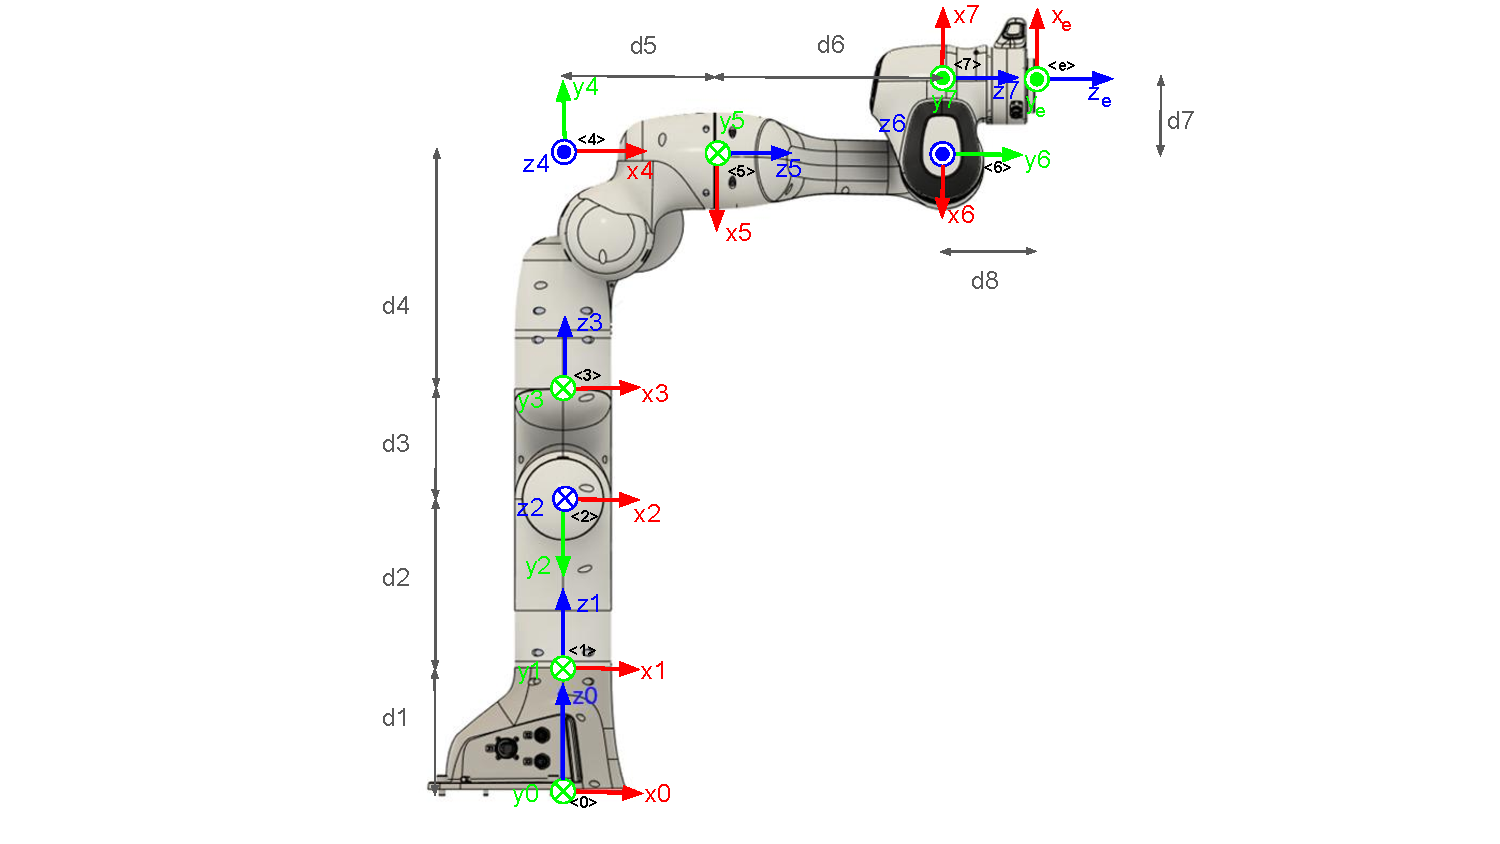
\includegraphics[width=1\linewidth]{Resources/franka.pdf}
\caption{exercise 5 frames}
\label{fig:ex2}
\end{figure}

Figure \ref{fig:ex2} shows the frame tree for the 7 joints of the Franka robot. With reference to the figure, use the geometric definition of the transformation matrix to compute by hand the following matrices.
\begin{itemize}
\item \textbf{Q5.1} \hspace{10mm} $^0_1 T$
\item \textbf{Q5.2} \hspace{10mm} $^1_2 T$
\item \textbf{Q5.3} \hspace{10mm} $^2_3 T$
\item \textbf{Q5.4} \hspace{10mm} $^3_4 T$
\item \textbf{Q5.5} \hspace{10mm} $^4_5 T$
\item \textbf{Q5.6} \hspace{10mm} $^5_6 T$
\item \textbf{Q5.7} \hspace{10mm} $^6_7 T$
\item \textbf{Q5.8} \hspace{10mm} $^7_e T$
\end{itemize}

You \textbf{MUST} compute the matrices \textbf{WITHOUT} using mathematical software.

\newpage
\section{Exercise 1} \label{P1}
% Write some intro
\subsection{Q1.1}
The \textit{AngleAxisToRot} is a function that, compute the \textit{rotation matrix} $\mathbf{R}$ with Rodrigues' formula 
\begin{equation}
	\mathbf{R} = \mathbf{I}_{3\times 3} + \sin{\theta}[\mathbf{h}\times] + (1 - \cos \theta)[\mathbf{h}\times]^2
	\label{eq::rodriguesformula}
\end{equation}
Given the \textit{axis of rotation} $\mathbf{h}$, which checked if it is a unit vector, can be considered three different cases for Equation \ref{eq::rodriguesformula} due to the values of \textit{angle of rotation} $\theta$:
\begin{itemize}
	\item $\theta = 0 \Rightarrow \mathbf{R} = \mathbf{I}_{3\times 3}$\space;
	\item $\theta = \pi \Rightarrow \mathbf{R} = \mathbf{I}_{3\times 3} + 2 [\mathbf{h}\times]^2$ where the square of a skew-symmetric matrix is $[\mathbf{h}\times]^2 = (\mathbf{h}\mathbf{h}^T -\mathbf{I}_{3\times 3})$\space;
	\item $\theta \in (0, \pi)$ where, since there are not simplifications of Equation \ref{eq::rodriguesformula} was needed to compute the axis of rotation's skew-symmetric matrix
		\begin{equation*}
			[\mathbf{h}\times] = \begin{bmatrix}
				0 & -h_3 & h_2 \\
				h_3 & 0 & -h_1 \\
				-h_2 & h_1 & 0
			\end{bmatrix}
	\end{equation*}
\end{itemize}

\subsection{Q1.2}
In the first case $\mathbf{h} = [1, 0, 0]^T$ and $\theta = \pi/2$ represent a $90$-degree rotation around the $x$-axis. In fact, $\mathbf{R}= \mathbf{R}_z\mathbf{R}_y\mathbf{R}_x =\mathbf{I}_{3\times 3}\mathbf{I}_{3\times 3}\mathbf{R}_x = \mathbf{R}_x$ where
\begin{equation*}
	\mathbf{R}_x = \begin{bmatrix}
				1 & 0 & 0 \\
				0 & 0 & -1 \\
				0 & 1 & 0
			\end{bmatrix}
\end{equation*}
\subsection{Q1.3}
In this configuration, which $\mathbf{h} = [0, 0, 1]^T$ and $\theta = \pi/3$, likely the previous case, it is a rotation around the $z$-axis but of $60$-degree
\begin{equation*}
	\mathbf{R}_z = \begin{bmatrix}
				\frac{1}{2} & -\frac{\sqrt{3}}{2} & 0 \\
				\frac{\sqrt{3}}{2} & \frac{1}{2} & 0 \\
				0 & 0 & 1
			\end{bmatrix}
\end{equation*}

\subsection{Q1.4}
For the last case, $\mathbf{\rho} = [-\pi/3, -\pi/6 ,\pi/3]$, before to call the function \textit{AngleAxisToRot} have been computed $\mathbf{h}$ and $\theta$ knowing that $\mathbf{\rho} = \theta\mathbf{h}$, and by definition $\parallel \mathbf{h} \parallel = 1$ this entail $\parallel \mathbf{\rho} \parallel = \parallel \theta \mathbf{h} \parallel = \theta \parallel \mathbf{h} \parallel = \theta$.
\begin{equation*}
	\theta = \sqrt{\rho _x^2 +\rho _y^2 +\rho _z^2} = \frac{\pi}{2} \qquad \mathbf{h} = \frac{\rho}{\theta} = [-\frac{2}{3},-\frac{1}{3},\frac{2}{3}]^T
\end{equation*}
This means that $R$ is a $90$-degree rotation around the vector $h$.
\begin{equation*}
	\mathbf{R} = \begin{bmatrix} 
		\frac{4}{9} & -\frac{4}{9} & -\frac{7}{9} \\
		\frac{8}{9} & \frac{1}{9} & \frac{4}{9} \\
		-\frac{1}{9} & -\frac{8}{9} & \frac{4}{9} 
	\end{bmatrix}
\end{equation*}

\section{Exercise 2} \label{P2}

\subsection{Q2.1}
\label{subsec::q12}
The \textit{RotToAngleAxis} function takes $\mathbf{R}$ and computes $\mathbf{h}$ and $\theta$. Before computing $\mathbf{R}$ were done three preliminary checks: $\mathbf{R}$ must be a $3\times 3$ matrix, $\det \mathbf{R} = 1$, and $\mathbf{R}\mathbf{R}^T = \mathbf{I}_{3\times 3}$.
Due to prevent floating point, e.g. Subsection \ref{subsec::q23}, was important implementing a tolerance for the computation of $\det \mathbf{R}$ and $\mathbf{R}\mathbf{R}^T = \mathbf{I}_{3\times 3}$\space, we have chosen a value of $10^{-10}$. Considering the
\begin{gather*}
	\text{Tr} R = \text{Tr}(\mathbf{I}_{3\times 3} + \sin{\theta}[\mathbf{h}\times] + (1 - \cos \theta)[\mathbf{h}\times]^2) = 1 + 2 \cos \theta \\
	\Rightarrow \theta = \arccos \Bigg ( \frac{\text{Tr} R -1}{2} \Bigg )
\end{gather*}
and the \textit{axial vector}
\begin{gather*}
	\mathbf{a} = \sin \theta \cdot \mathbf h = \text{Vex}\Bigg (\frac{\mathbf{R}\mathbf{R}^T}{2} \Bigg ) \\
	\Rightarrow \mathbf{h} = \frac{\mathbf{a}}{\sin \theta}
\end{gather*}
Notice that $theta$ could be equal to zero or $\pi$:
\begin{itemize}
	\item $\theta = 0$: in this case $\mathbf{h}$ can be arbitrary than we decided to rise an error.
	\item $\theta = \pi$: this represent a rotation of $180$-degree around one of the axes. In order to find $\mathbf{h}$, the script compute one
	\begin{equation*}
		h_i = \pm\sqrt{\frac{r_{ii}+1}{2}} \quad i \in \mathbb{N} \smallsetminus \{0\}, i \leq 3
	\end{equation*}
	Determinate the signs of other components $h_j$ ($j \in \mathbb{N} \smallsetminus \{0\}, j \leq 3$, $i\neq j$)
	 \begin{equation*}
	 	h_j = \text{sgn}(h_i) \text{sgn} (r_{ij})\sqrt{\frac{r_{jj}+1}{2}}
	 \end{equation*}
	 This let us to find the two possible configurations of the vector $\mathbf{h}$.
\end{itemize}
\subsection{Q2.2} 
The rotation matrix
\begin{equation*}
	R = \begin{pmatrix}
        1& 0 & 0 \\
        0 & 0 & -1 \\
        0 & 1 & 0
    \end{pmatrix}
\end{equation*}
rappresents a rotation around $x$-axis. In fact, the function returns $\mathbf{h} = [1,0,0]^T$ and $\theta = \frac{\pi}{2}$.
\subsection{Q2.3} \label{subsec::q23}
In this case the rotation is around the $z$-axis, as show in the rotation matrix
\begin{equation*}
	R = \begin{pmatrix}
		\frac{1}{2}& -\frac{\sqrt{3}}{2} & 0 \\
		\frac{\sqrt{3}}{2} & \frac{1}{2} & 0 \\
		0 & 0 & 1
	\end{pmatrix}
\end{equation*}
Since it’s clear that $\arccos(\frac{1}{2})=\arcsin(\frac{\sqrt{3}}{2})= \frac{\pi}{3}$, then $\mathbf{h} = [0,0,1]^T$ and $\theta = \frac{\pi}{3}$. 
\subsection{Q2.3}
In the third case, $R = I_{3\times 3}$, it means there is no rotation, then $\mathbf{h}$ is arbitrary.
\subsection{Q2.4}
With the rotation matrix 
\begin{equation*}
	R = \begin{pmatrix}
		-1& 0 & 0 \\
		0 & -1 & 0 \\
		0 & 0 & 1
	\end{pmatrix}
\end{equation*}
the angle of rotation $\theta = \pi$, this mean that there are two possible configurations of the vector $\mathbf{h} \rightarrow \mathbf{h}_+= [0,0,1]^T$, $\mathbf{h}_-= [0,0,-1]^T$.
\section{Exercise 3} \label{P3}

\subsection{Q3.1}
The \textit{YPRToRot} function computes $\mathbf{R}$ using the \textit{Yaw-Pitch-Roll} representation
\begin{gather}
	\mathbf{R}_\text{YPR} = \mathbf{R}_z(\psi)\mathbf{R}_y(\theta)\mathbf{R}_x(\phi) = \nonumber \\ = \begin{bmatrix}
\cos\psi \cos\theta & \cos\psi \sin\theta \sin\phi - \sin\psi \cos\phi & \cos\psi \sin\theta \cos\phi + \sin\psi \sin\phi \\
\sin\psi \cos\theta & \sin\psi \sin\theta \sin\phi + \cos\psi \cos\phi & \sin\psi \sin\theta \cos\phi - \cos\psi \sin\phi \\
-\sin\theta & \cos\theta \sin\phi & \cos\theta \cos\phi
\end{bmatrix}
\end{gather}
After the \textit{rotation matrix} was checked as in Subsection \ref{subsec::q12}.
\subsection{Q3.2}
We have given to the function the inputs $\psi = 0, \theta = 0, \phi = \frac{\pi}{2}$, it means that  $\mathbf{R}_z(\psi) = \mathbf{R}_y(\theta) = \mathbf{I}_{3 \times 3} $ then there will be no rotation around $Z$ and $Y$ axes. The only rotational contribution is around $x$-axis.
\begin{gather}
	\mathbf{R}_\text{YPR} = \mathbf{R}_x(\phi) \nonumber = \begin{pmatrix}
	 1& 0 & 0 \\
	0 & 0 & -1 \\
	0 & 1 & 0
	\end{pmatrix}
\end{gather} 
\subsection{Q3.3}
The angles' composition $\psi = \frac{\pi}{3}, \theta = 0, \phi = 0$, as discussed above has only the rotational contribution around $z$-axis.
\begin{equation*}
\mathbf{R}_\text{YPR} =	\mathbf{R}_z(\psi) = \begin{pmatrix}
        \frac{1}{2}& -\frac{\sqrt{3}}{2} & 0 \\
        \frac{\sqrt{3}}{2} & \frac{1}{2} & 0 \\
        0 & 0 & 1
    \end{pmatrix} 
\end{equation*}
\subsection{Q3.4}
The third case with those three input angles $\psi = \frac{\pi}{3}, \theta = \frac{\pi}{2}, \phi = \frac{\pi}{4}$ is a rotation around all the three axes. The result is the following
\begin{equation*}
	\mathbf{R}_\text{YPR} = \begin{pmatrix}
	 0& \frac{\sqrt{6}}{4} -\frac{\sqrt{2}}{4} & \frac{\sqrt{6}}{4} + \frac{\sqrt{2}}{4}\\
	0 & \frac{\sqrt{6}}{4} + \frac{\sqrt{2}}{4} & \frac{\sqrt{6}}{4} -\frac{\sqrt{2}}{4}  \\
	-1 & 0 & 0
	\end{pmatrix} 
\end{equation*}
\subsection{Q3.5}
The parameters are $\psi = 0, \theta = \frac{\pi}{2}, \phi = -\frac{\pi}{12}$ means that there is no rotation around $z$-axis. In fact, the rotation matrix has the contributes of rotation around $y$ and $x$ axes.
\begin{equation*}
	\mathbf{R}_\text{YPR} = \mathbf{R}_y(\theta)\mathbf{R}_x(\phi) 
	= \begin{pmatrix}
	0 & -\frac{\sqrt{6} - \sqrt{2}}{4} & \frac{\sqrt{6} + \sqrt{2}}{4} \\ 0 & \frac{\sqrt{6} + \sqrt{2}}{4} & \frac{\sqrt{6} - \sqrt{2}}{4} \\ -1 & 0 & 0 \\ 
	\end{pmatrix} 
\end{equation*}

\section{Exercise 4} \label{P4}

\subsection{Q4.1}
The \textit{RotToYPR} function compute a possible configuration of the angles $\psi$, $\theta$, and $\phi$ from a \textit{Yaw-Pitch-Roll matrix}. After doing the same checks, reported in Subsection \ref{subsec::q12}, to verify if the given matrix is a rotation matrix, the script compute angles as
\begin{gather*}
	\theta = \texttt{arctan2} \big (-r_{31} \texttt{,} \sqrt{r_{11}^2+r_{21}^2}\big ) \\
	\psi = \texttt{arctan2} (r_{21} \texttt{,} r_{11}) \\
	\phi = \texttt{arctan2} (r_{32} \texttt{,} r_{33})
\end{gather*}
checking if the configuration is not singular ($\cos \theta \neq 0$). Notice that $r_{ij}$ ($i,j \in \mathbb{N}\small\backslash\{0\}, i \leq 3, j \leq 3$)
\subsection{Q4.2}
The matrix $\mathbf{R}$ passed to the function and the respective output angles are shown below
\begin{gather*}
	\mathbf{R}= \begin{pmatrix}
		1& 0 & 0 \\
		0 & 0 & -1 \\
		0 & 1 & 0
	\end{pmatrix} \Rightarrow
	\psi = 0,\, 
	\theta = 0,\,\phi = \frac{\pi}{2} 
\end{gather*}
It is evident that the matrix $\mathbf{R}$ corresponds to an $\mathbf{R}_x(\phi)$ matrix, as confirmed by the fact that only the angle $\phi$, characteristic of rotation along the $x$-axis, is different from zero.
\subsection{Q4.3}
In this case the input and the respective output angles are
\begin{gather*}
	\mathbf{R}= \begin{pmatrix}
		\frac{1}{2}& -\frac{\sqrt{3}}{2} & 0 \\
		\frac{\sqrt{3}}{2} & \frac{1}{2} & 0 \\
		0 & 0 & 1
	\end{pmatrix} \Rightarrow
	\psi = \frac{\pi}{3},\,
	\theta = 0,\,
	\phi = 0
\end{gather*}
They represent a rotation around the $z$-axis.
\subsection{Q4.4}
As represented in
\begin{gather*}
	\mathbf{R}= \begin{pmatrix}
		0 & -\frac{\sqrt{2}}{2} & \frac{\sqrt{2}}{2} \\
		\frac{1}{2} & \frac{\sqrt{2}\sqrt{3}}{4} & \frac{\sqrt{2}\sqrt{3}}{4} \\
		-\frac{\sqrt{3}}{2} & \frac{\sqrt{2}}{4} & \frac{\sqrt{2}}{4}
	\end{pmatrix} \Rightarrow
	\psi = \frac{\pi}{2},\,
	\theta = \frac{\pi}{3},\,
	\phi = \frac{\pi}{4}
\end{gather*}
The rotation matrix $\mathbf{R}$ is a composition of three rotation, one for each axis.
\section{Exercise 5} \label{P5}
\subsection{Q5.1}
\begin{gather}
	^0_1 T = \begin{pmatrix}
        1 & 0 & 0 & 0 \\
        0 & 1 & 0 & 0 \\
        0 & 0 & 1 & d_1 \\
        0 & 0 & 0 & 1
    \end{pmatrix} \quad
    ^1_2 T = \begin{pmatrix}
        1 & 0 & 0 & 0 \\
        0 & 0 & 1 & 0 \\
        0 & -1 & 0 & d_2 \\
        0 & 0 & 0 & 1
    \end{pmatrix} \quad
    ^2_3 T = \begin{pmatrix}
        1 & 0 & 0 & 0 \\
        0 & 0 & -1 & 0 \\
        0 & 1 & 0 & d_3 \\
        0 & 0 & 0 & 1
    \end{pmatrix} \quad
    ^3_4 T = \begin{pmatrix}
        1 & 0 & 0 & 0 \\
        0 & 0 & -1 & 0 \\
        0 & 1 & 0 & d_4 \\
        0 & 0 & 0 & 1
    \end{pmatrix} \nonumber \\
    \nonumber \\
    ^4_5 T = \begin{pmatrix}
        0 & 1 & 0 & d_5 \\
        0 & 0 & 1 & 0 \\
        1 & 0 & 0 & 0 \\
        0 & 0 & 0 & 1
    \end{pmatrix} \quad
    ^5_6 T = \begin{pmatrix}
        1 & 0 & 0 & 0 \\
        0 & 0 & -1 & 0 \\
        0 & 1 & 0 & d_6 \\
        0 & 0 & 0 & 1
    \end{pmatrix} \quad
    ^6_7 T = \begin{pmatrix}
        1 & 0 & 0 & -d_7 \\
        0 & 0 & 1 & 0 \\
        0 & 0 & 0 & 0 \\
        0 & 0 & 0 & 1
    \end{pmatrix} \quad
    ^7_e T = \begin{pmatrix}
        1 & 0 & 0 & 0 \\
        0 & 1 & 0 & 0 \\
        0 & 0 & 1 & d_8 \\
        0 & 0 & 0 & 1
    \end{pmatrix} \nonumber
\end{gather}

\pagebreak

\section{Appendix}
\textit{[Comment] Add here additional material (if needed)} 
\subsection{Appendix A}

\subsection{Appendix B}


\end{document}
